\documentclass[12pt, aspectratio=169]{beamer}
\usepackage{
    hyperref,
    graphicx,
    % enumitem,
    transparent,
    siunitx,
    pgfpages,
    caption,
    booktabs,
    multirow,
    bm,
    standalone,
    tikz,
    comment,
    xcolor,
    svg,
}
\usepackage[hang,flushmargin]{footmisc}
\setbeameroption{hide notes}
% \setbeameroption{show only notes}
% \setbeameroption{show notes on second screen}
\setbeamertemplate{note page}[plain]
\setbeamercovered{transparent}

% get rid of junk
\usetheme{default}
\usecolortheme{orchid}
\beamertemplatenavigationsymbolsempty
\hypersetup{pdfpagemode=UseNone} % don't show bookmarks on initial view

% named colors
\definecolor{offwhite}{RGB}{249,242,215}
\definecolor{foreground}{RGB}{255,255,255}
\definecolor{background}{RGB}{24,24,24}
\definecolor{title}{RGB}{107,174,214}
\definecolor{gray}{RGB}{155,155,155}
\definecolor{subtitle}{RGB}{102,255,204}
\definecolor{hilight}{RGB}{102,255,204}
\definecolor{vhilight}{RGB}{255,111,207}
\definecolor{lolight}{RGB}{155,155,155}
%\definecolor{green}{RGB}{125,250,125}

% use those colors
\setbeamercolor{titlelike}{fg=title}
\setbeamercolor{subtitle}{fg=subtitle}
\setbeamercolor{institute}{fg=gray}
\setbeamercolor{normal text}{fg=foreground,bg=background}
\setbeamercolor{item}{fg=foreground} % color of bullets
\setbeamercolor{subitem}{fg=foreground}
\setbeamercolor{itemize/enumerate subbody}{fg=foreground}
\setbeamercolor{section in toc}{fg=title}
\setbeamercolor{alerted text}{fg=title}

\setbeamertemplate{itemize subitem}{{\textendash}}
\setbeamerfont{itemize/enumerate subbody}{size=\footnotesize}
\setbeamerfont{itemize/enumerate subitem}{size=\footnotesize}

\addtobeamertemplate{block alerted begin}{%
  \setbeamercolor{alerted text}{fg=red}%
}{}
\addtobeamertemplate{block example begin}{%
  \setbeamercolor{alerted text}{fg=green}%
}{}

% add a bit of space at the top of the notes page
\addtobeamertemplate{note page}{\setlength{\parskip}{12pt}}

% a few macros
\setbeamertemplate{description item}{
    \hfill\alert{\textbf{\insertdescriptionitem}}
}
\setbeamertemplate{itemize items}[circle]

\AtBeginSection[]{
    \begin{frame}
        \vfill
        \centering
        \Huge\color{title}\insertsectionhead
        \vfill
    \end{frame}
}

\newcommand\blfootnote[1]{%
    \begingroup
    \renewcommand\thefootnote{}\footnote{\tiny \color{lolight} #1}%
    \huge%
    \addtocounter{footnote}{-1}%
    \endgroup
}

% math macros
\renewcommand{\d}[1]{\mathsf{d}#1}
\newcommand{\diff}[2]{\frac{\mathsf{d} #1}{\mathsf{d} #2}}
\newcommand{\pdiff}[2]{\frac{\partial #1}{\partial #2}}
\newcommand{\Diff}[2]{\frac{\mathsf{D} #1}{\mathsf{D} #2}}
\renewcommand\vec{\bm}
\newcommand{\uvec}[1]{\vec{\hat{#1}}}
\newcommand{\grad}{\vec{\nabla}}
\newcommand{\prandtl}{\ensuremath{\mathsf{Pr}}}
\newcommand{\rayleigh}{\ensuremath{\mathsf{Ra}}}

% text macros
\newcommand{\rb}{Rayleigh-B\'{e}nard}

\title{
    Calculation and analysis of subgrid tendencies in a coarse model
    of \rb{} convection
}
\author{Thomas Schanzer}
\institute{
    Climate Change Research Centre and
    ARC Centre of Excellence for Climate Extremes \\
    \vspace{6pt}
    University of New South Wales, Sydney, Australia
}
\date{Thursday 28 September 2023}


\begin{document}

\begin{frame}
\maketitle
\end{frame}

\section{1. We can estimate small-scale effects using high-resolution data}

\begin{frame}
\centering
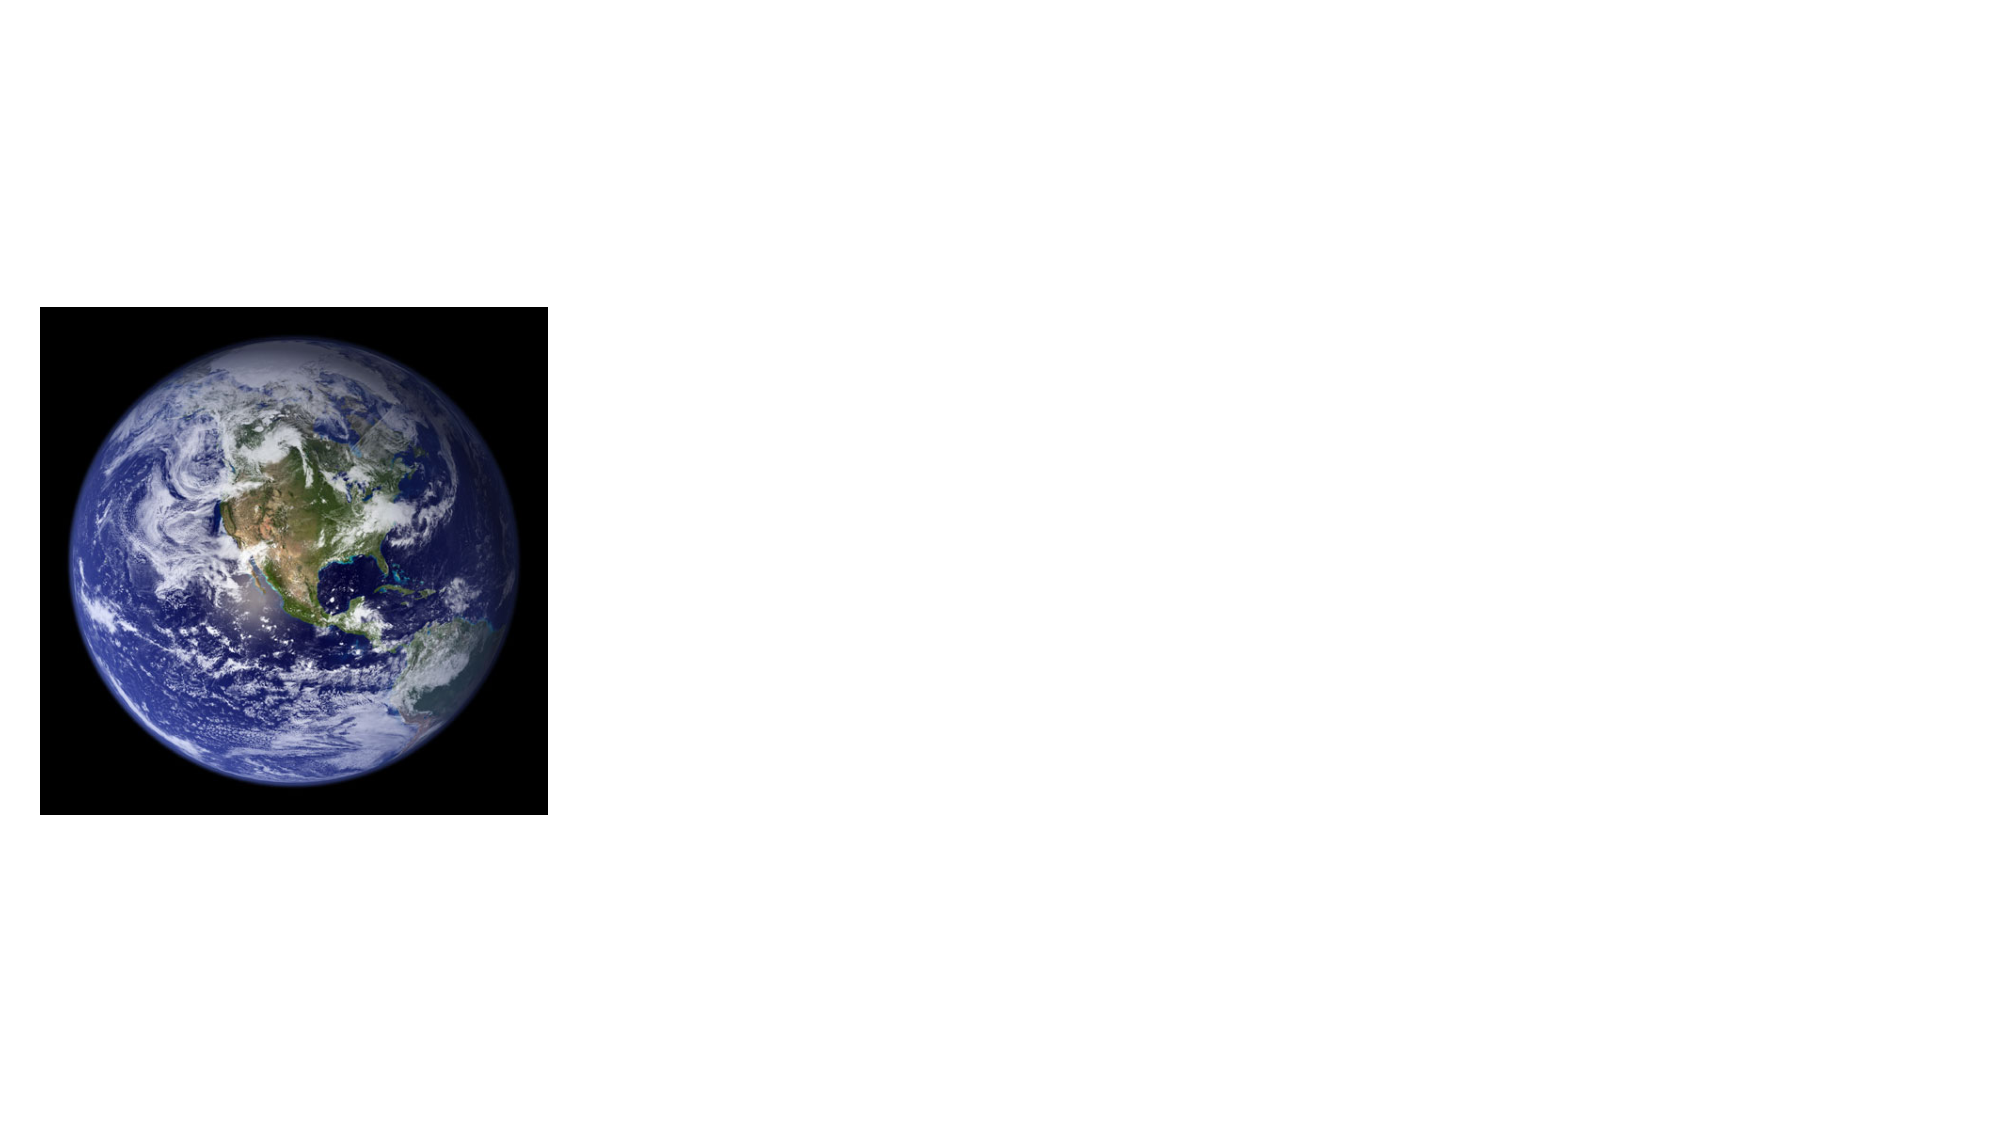
\includegraphics[width=\linewidth]{figures/introduction1.pdf}
\end{frame}

\begin{frame}
\centering
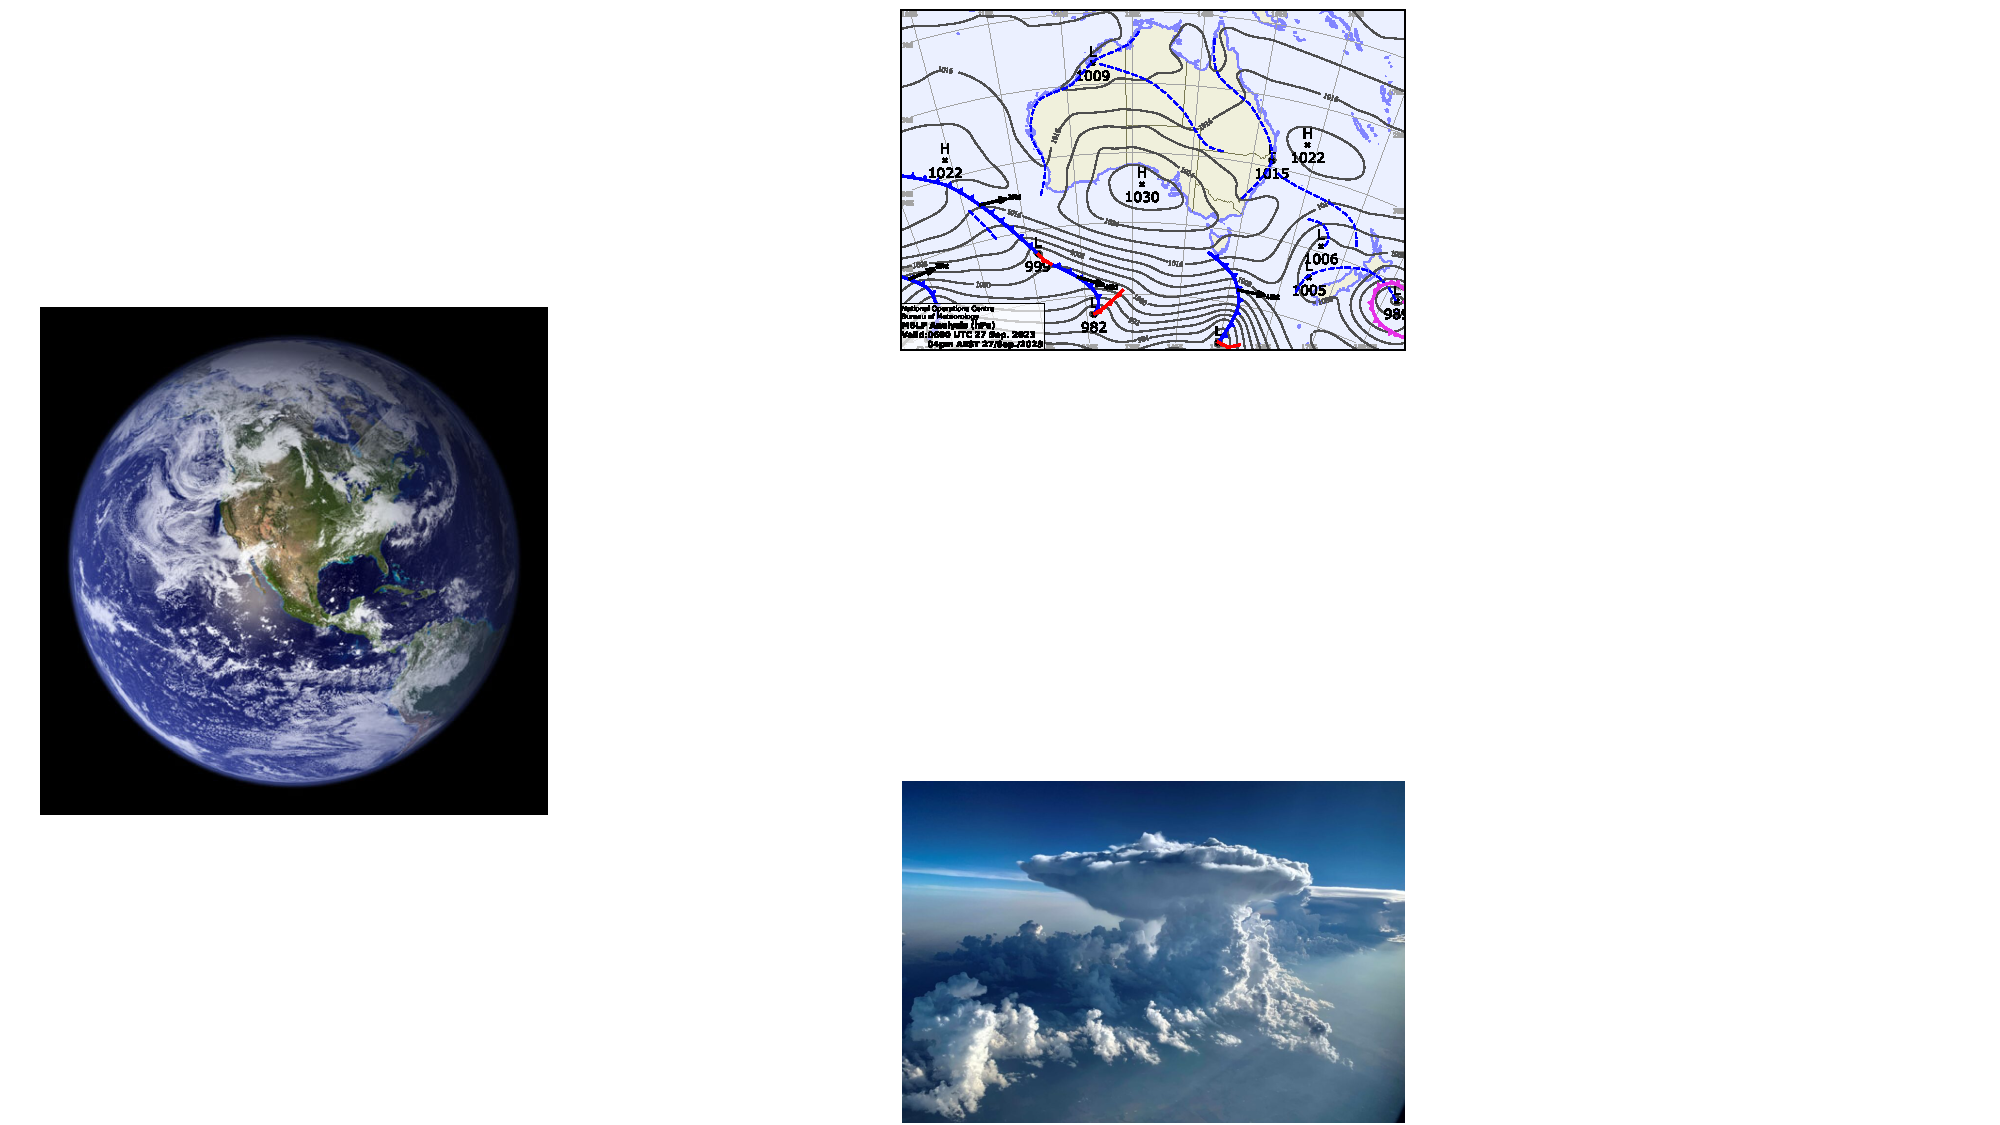
\includegraphics[width=\linewidth]{figures/introduction2.pdf}
\end{frame}

\begin{frame}
\centering
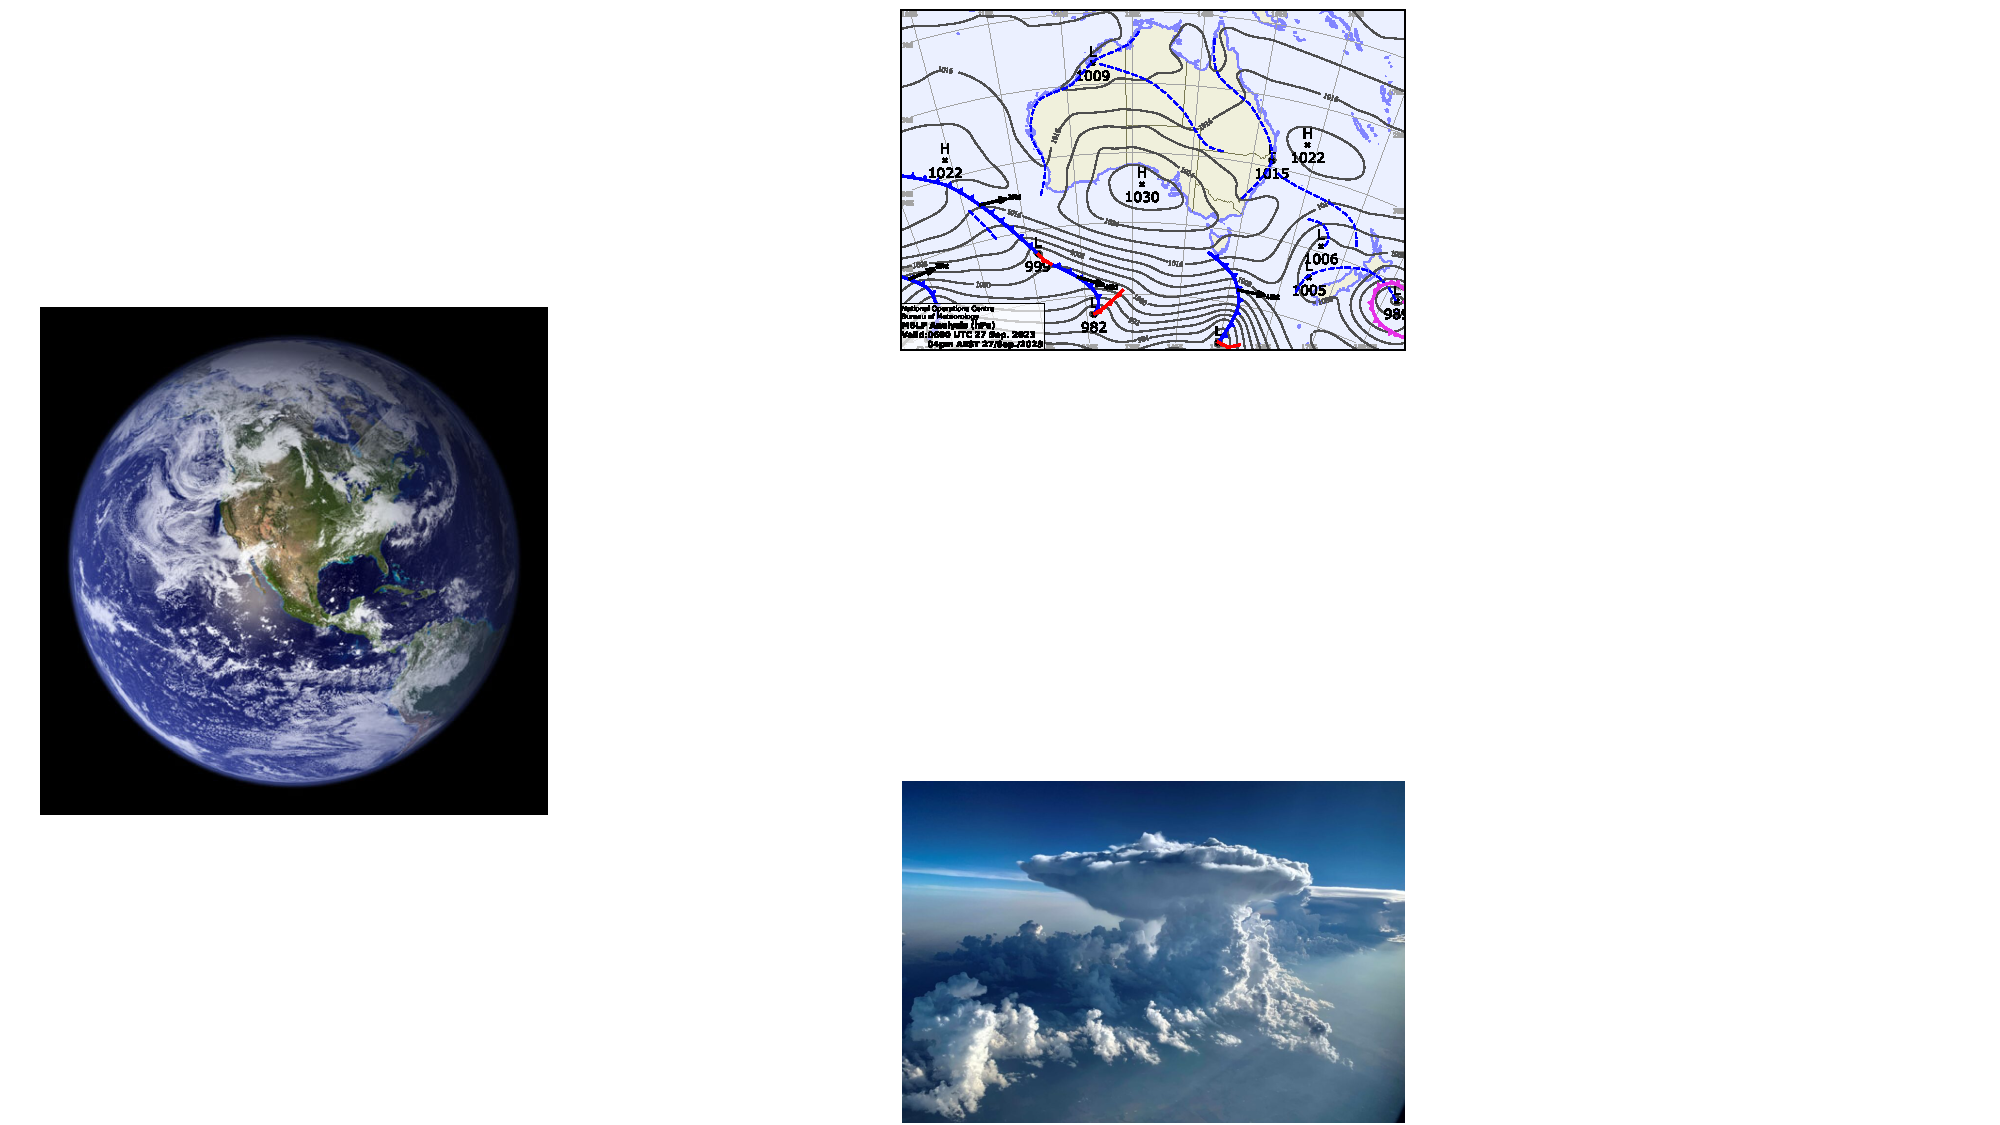
\includegraphics[width=\linewidth]{figures/introduction3.pdf}
\end{frame}

\begin{frame}
\centering
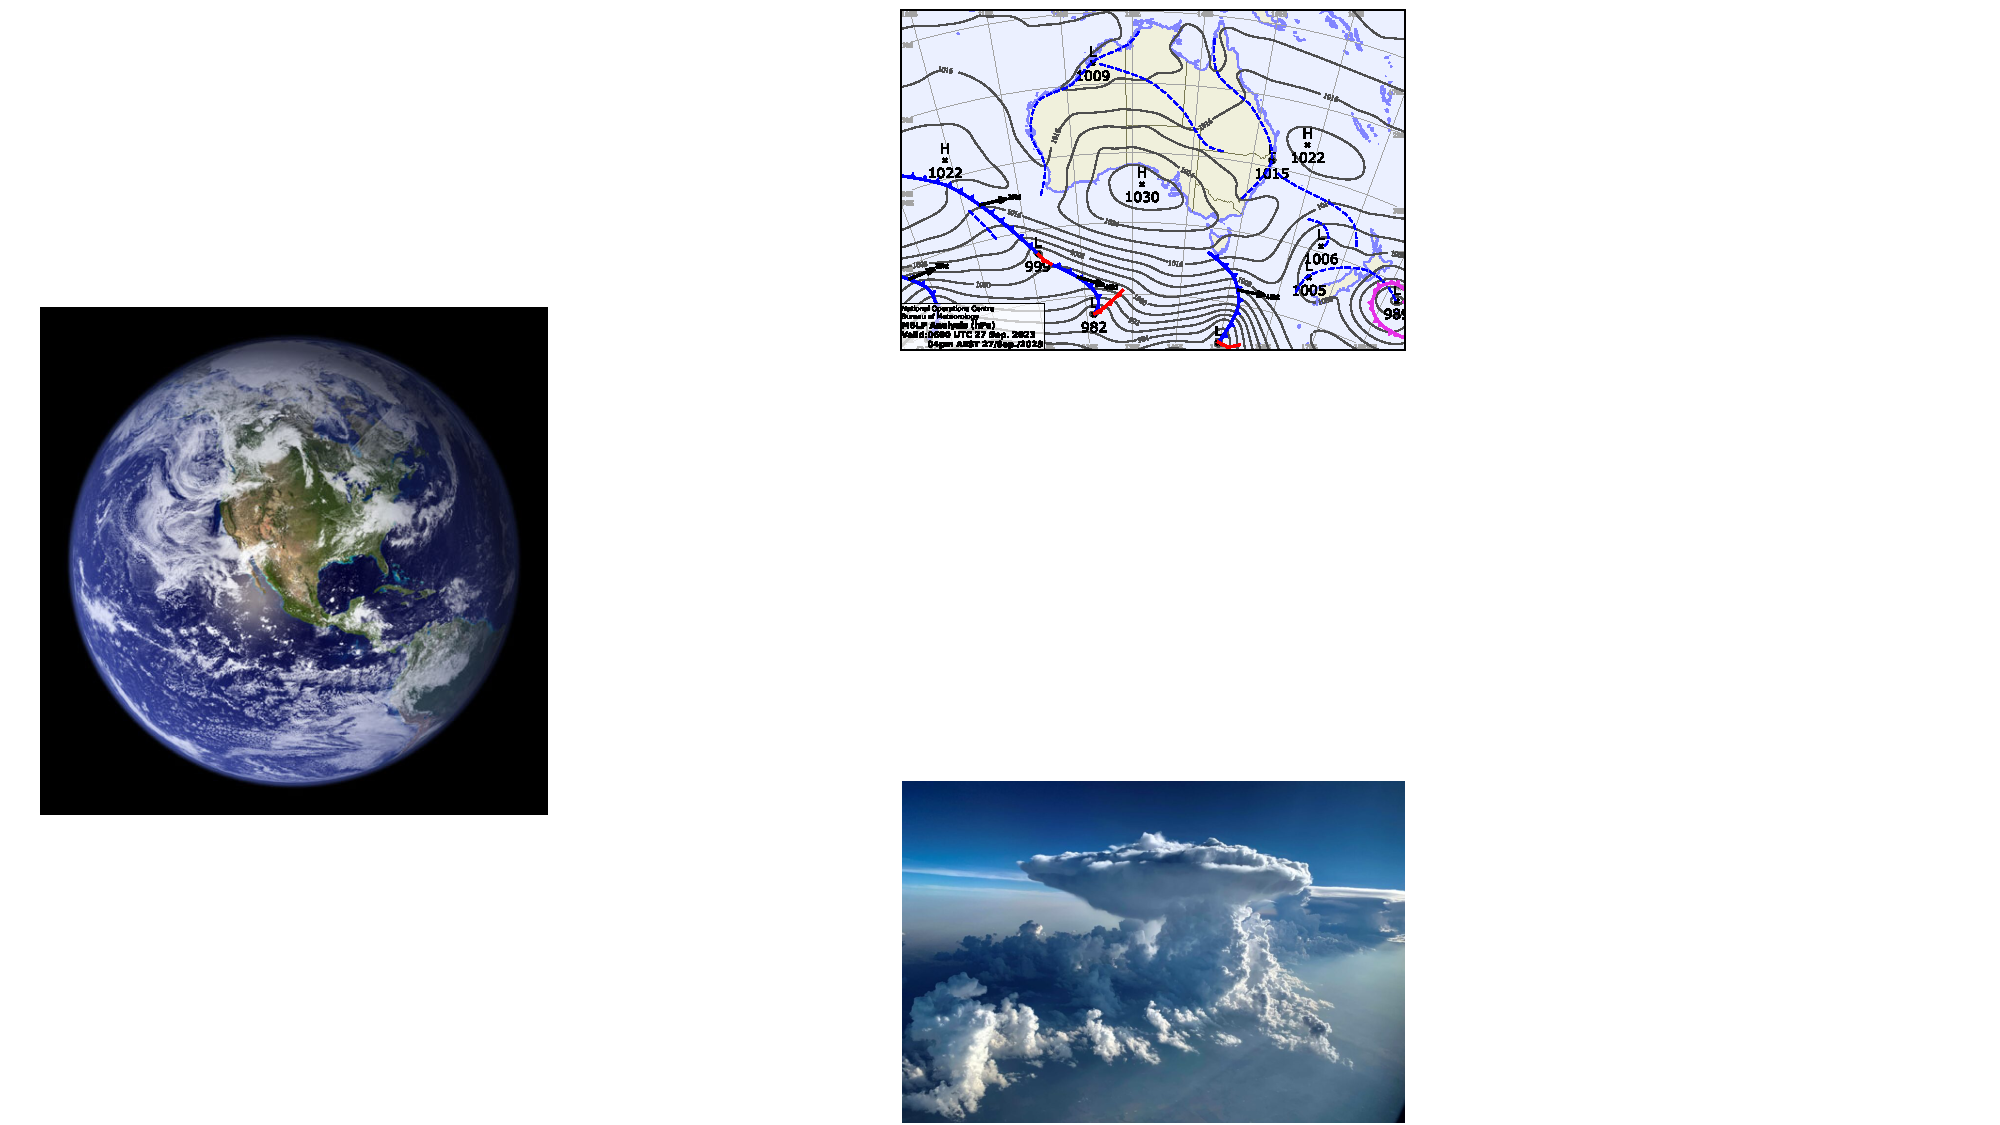
\includegraphics[width=\linewidth]{figures/introduction4.pdf}
\end{frame}

\begin{frame}
But we can't solve
\[
    \diff{\vec{x}}{t} = \vec{G}(\vec{x}) + \vec{C}(\vec{x}, \vec{y})!
\]
\vfill
We need a \emph{parametrised} system
\[
    \diff{\vec{x}}{t} \approx \vec{G}(\vec{x}) + \vec{P}(\vec{x}).
\]
\vfill
How can we estimate $\vec{C}(\vec{x}, \vec{y})$ without knowing $\vec{y}$?
\end{frame}

\begin{frame}
The decomposition $\vec{z} \to (\vec{x}, \vec{y})$ is achieved via
\[
    \vec{x} = \langle \vec{z} \rangle,
    \qquad \vec{y} = \vec{z} - \langle \vec{z} \rangle.
\]
\vfill
On the one hand,
\[
    \left \langle \diff{\vec{z}}{t} \right \rangle
    = \langle \vec{F}(\vec{z}) \rangle.
\]
\vfill
On the other hand,
\[
    \left \langle \diff{\vec{z}}{t} \right \rangle
    = \diff{\langle \vec{z} \rangle}{t}
    = \vec{G}(\langle \vec{z} \rangle)
        + \vec{C}(\langle \vec{z} \rangle, \vec{y}).
\]
\end{frame}

\begin{frame}
This means that
\[
    \vec{C}(\langle \vec{z} \rangle, \vec{y})
    = \langle \vec{F}(\vec{z}) \rangle - \vec{G}(\langle \vec{z} \rangle).
\]
\vfill
\begin{center}
    \alert{We can calculate the coupling using high-resolution data.}
\end{center}
\end{frame}

\section{2. Putting it into practice: \rb{} convection}

% RBC
\begin{frame}
2D \rb{} convection:
\begin{align*}
    \Diff{}{t} \begin{pmatrix} u \\ w \end{pmatrix}
        &= -\grad \pi + \nu \nabla^2 \begin{pmatrix} u \\ w \end{pmatrix}
        + \theta \uvec{z} \\[5pt]
    \Diff{\theta}{t}  &= \kappa \nabla^2 \theta \\[5pt]
    \grad \cdot \begin{pmatrix} u \\ w \end{pmatrix} &= 0
\end{align*}
\begin{itemize}
    \item No-slip, isothermal top/bottom boundaries
    \item Periodic lateral boundaries
    \item Solved using Dedalus (pseudospectral code in Python)
\end{itemize}
\end{frame}

% method flowchart with plots for illustration
\begin{frame}
\centering
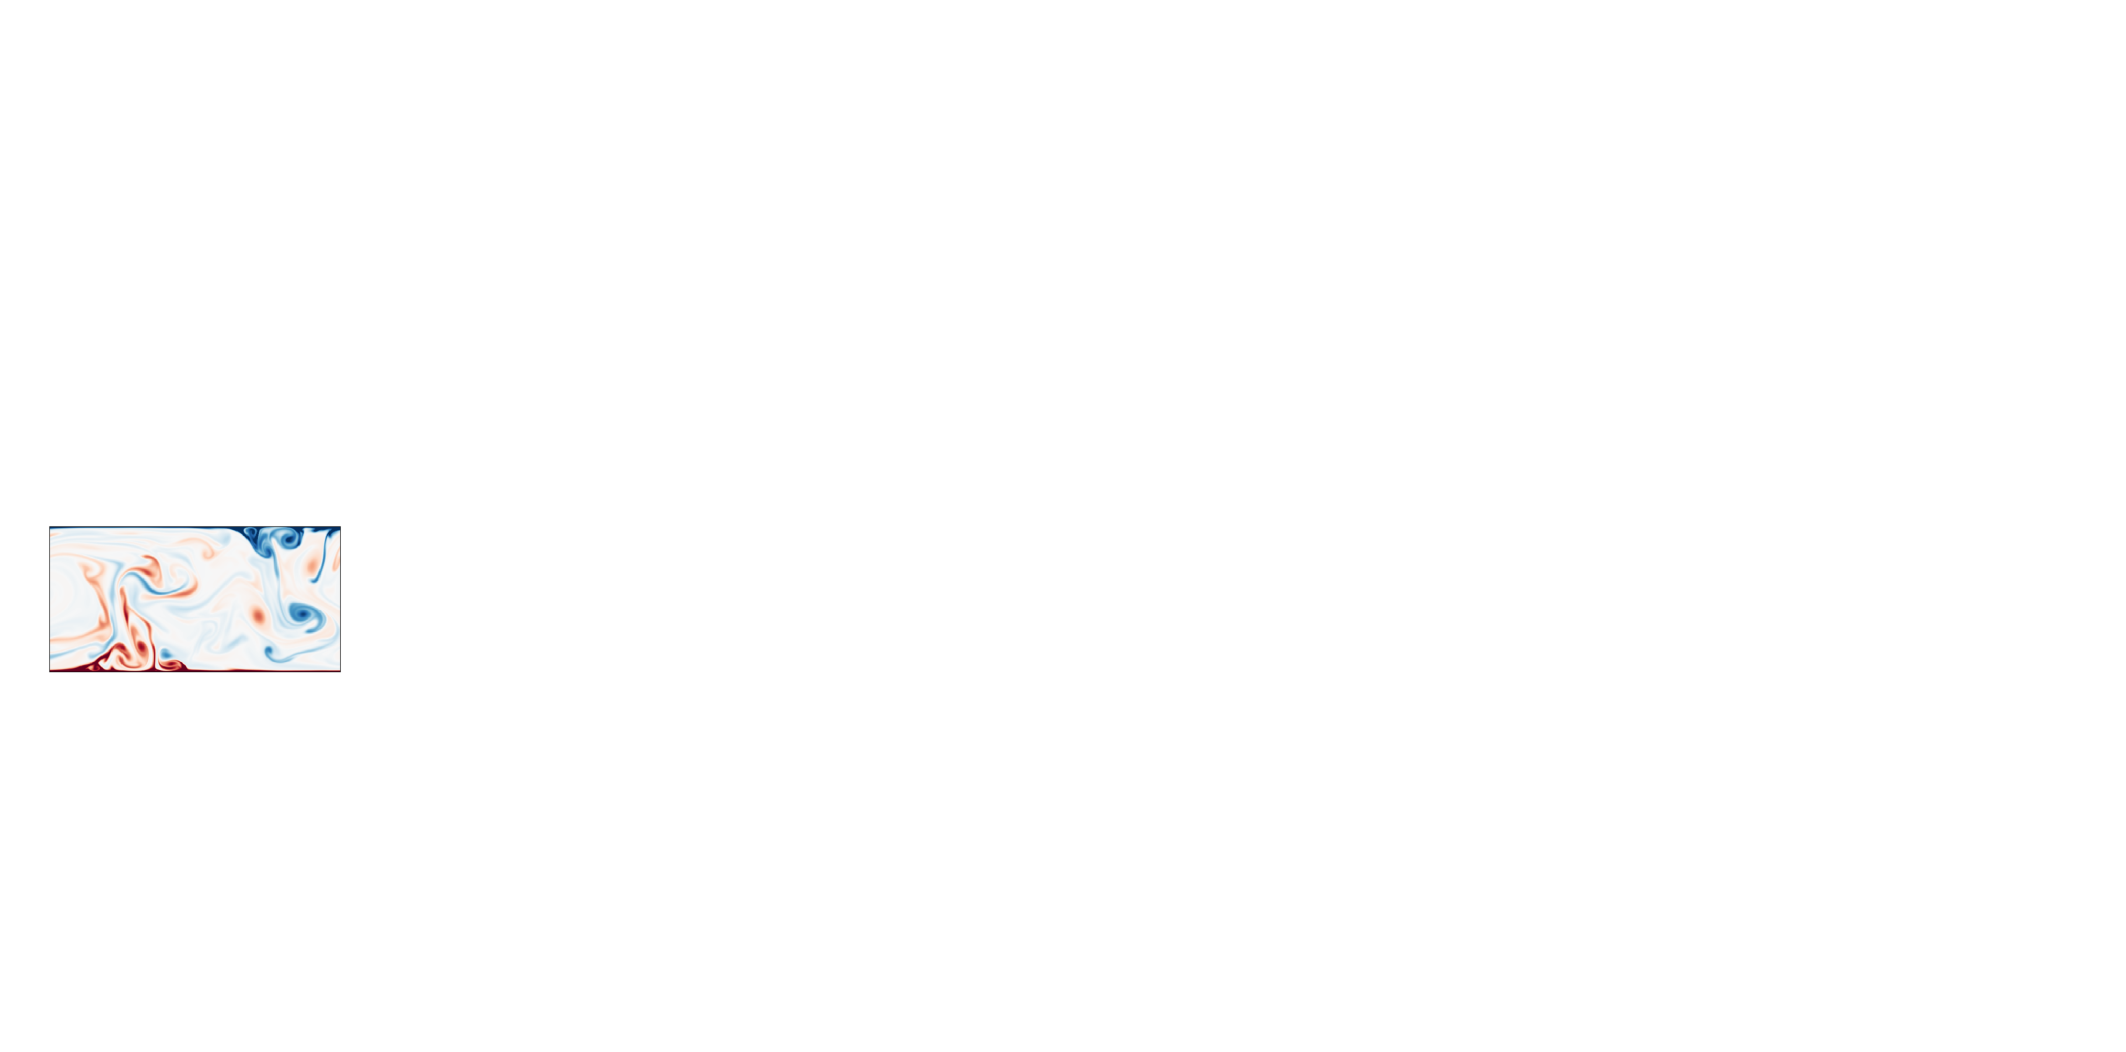
\includegraphics[width=\linewidth]{figures/method1.pdf}
\end{frame}

\begin{frame}
\centering
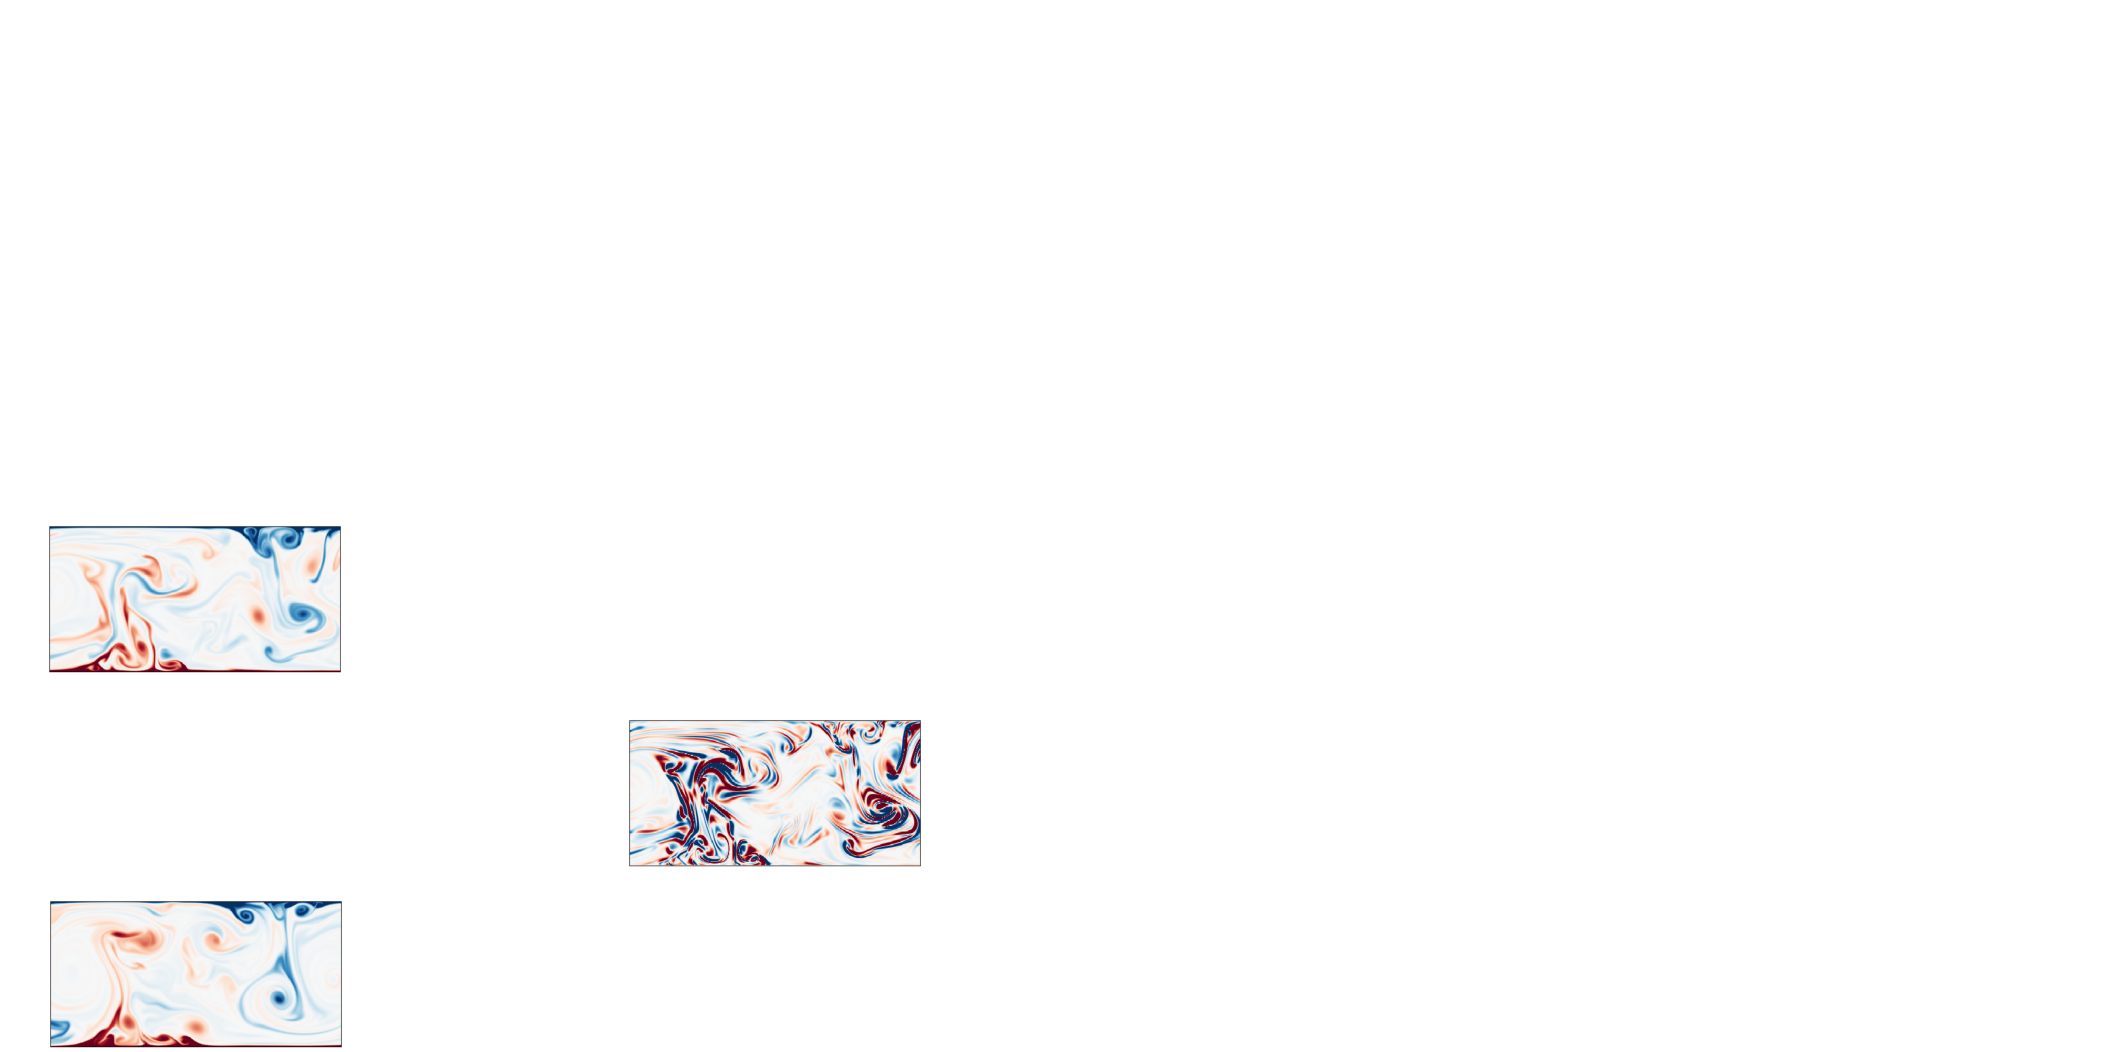
\includegraphics[width=\linewidth]{figures/method2.pdf}
\end{frame}

\begin{frame}
\centering
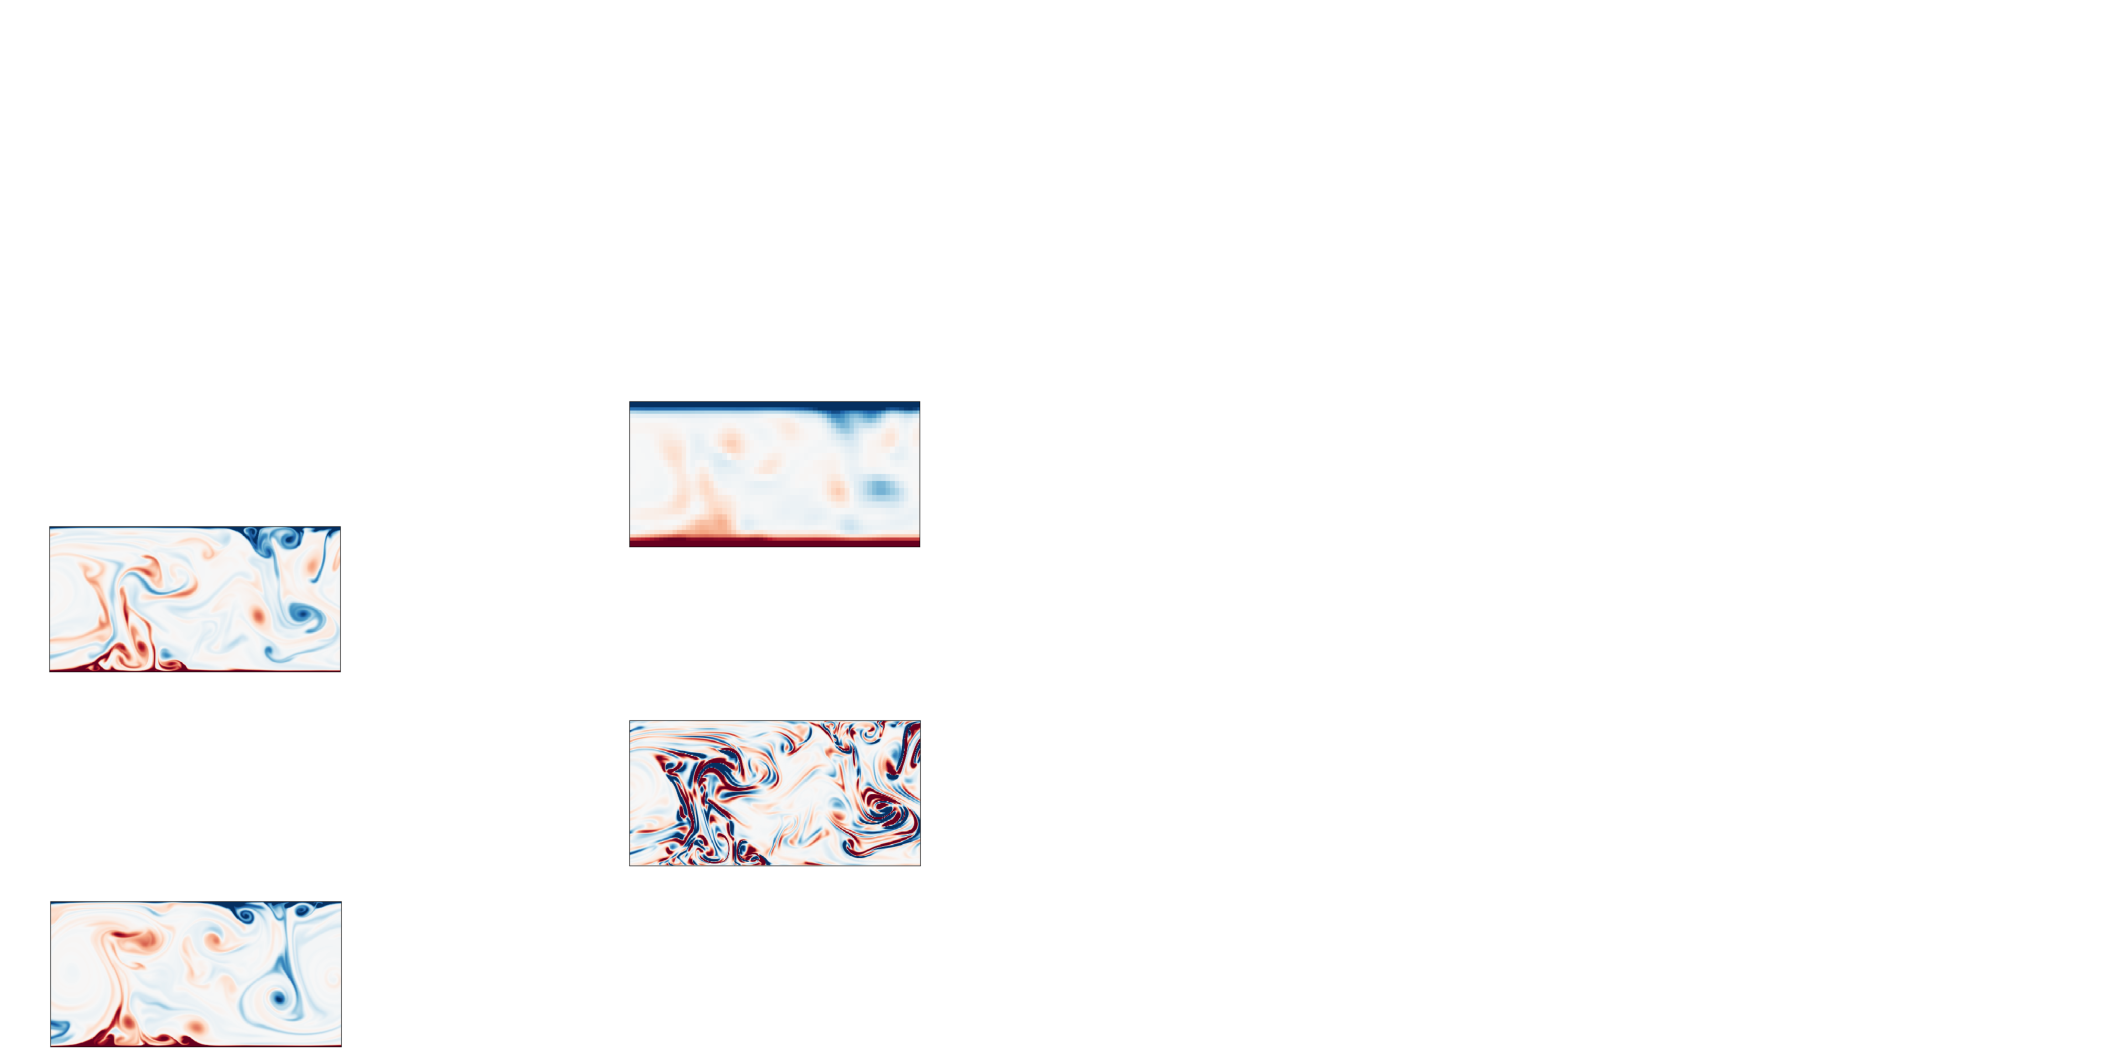
\includegraphics[width=\linewidth]{figures/method3.pdf}
\end{frame}

\begin{frame}
\centering
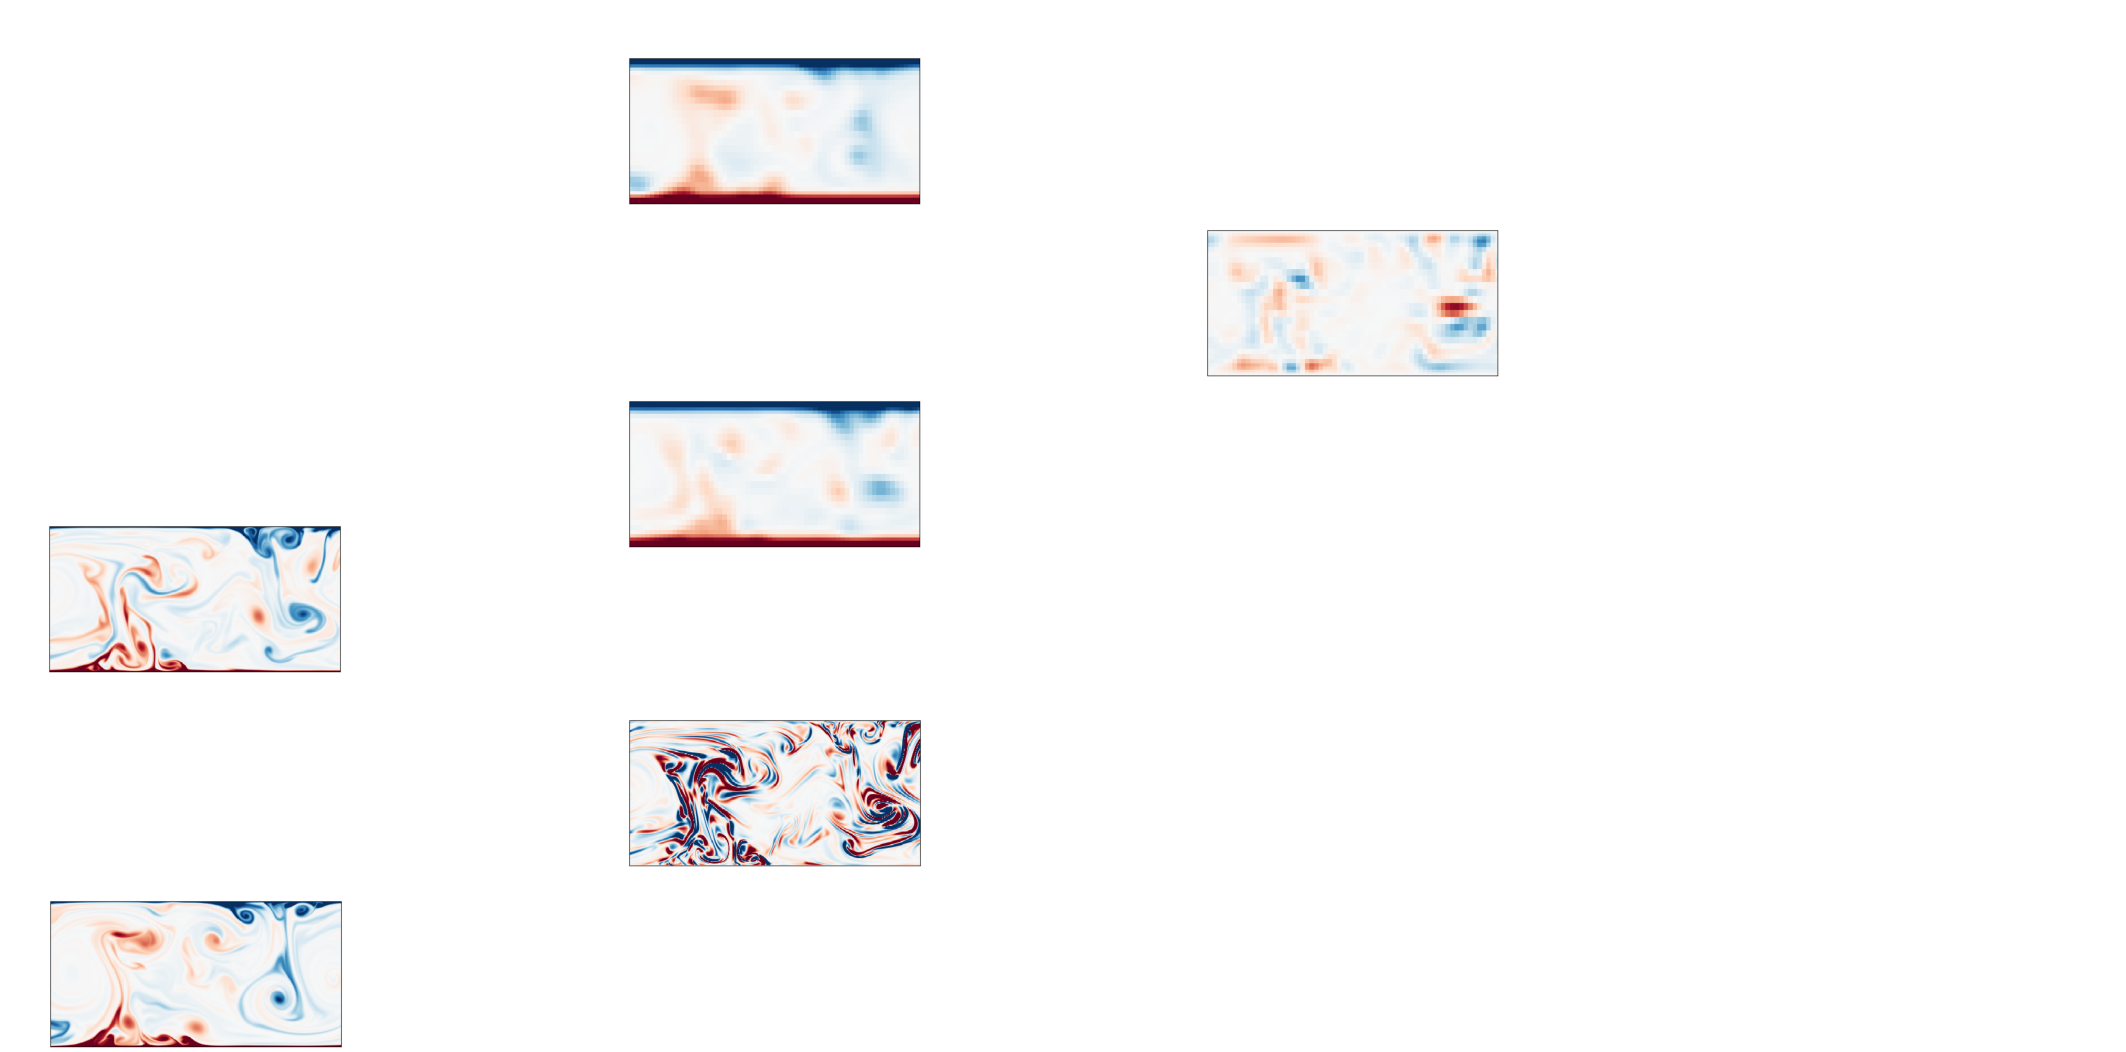
\includegraphics[width=\linewidth]{figures/method4.pdf}
\end{frame}

\begin{frame}
\centering
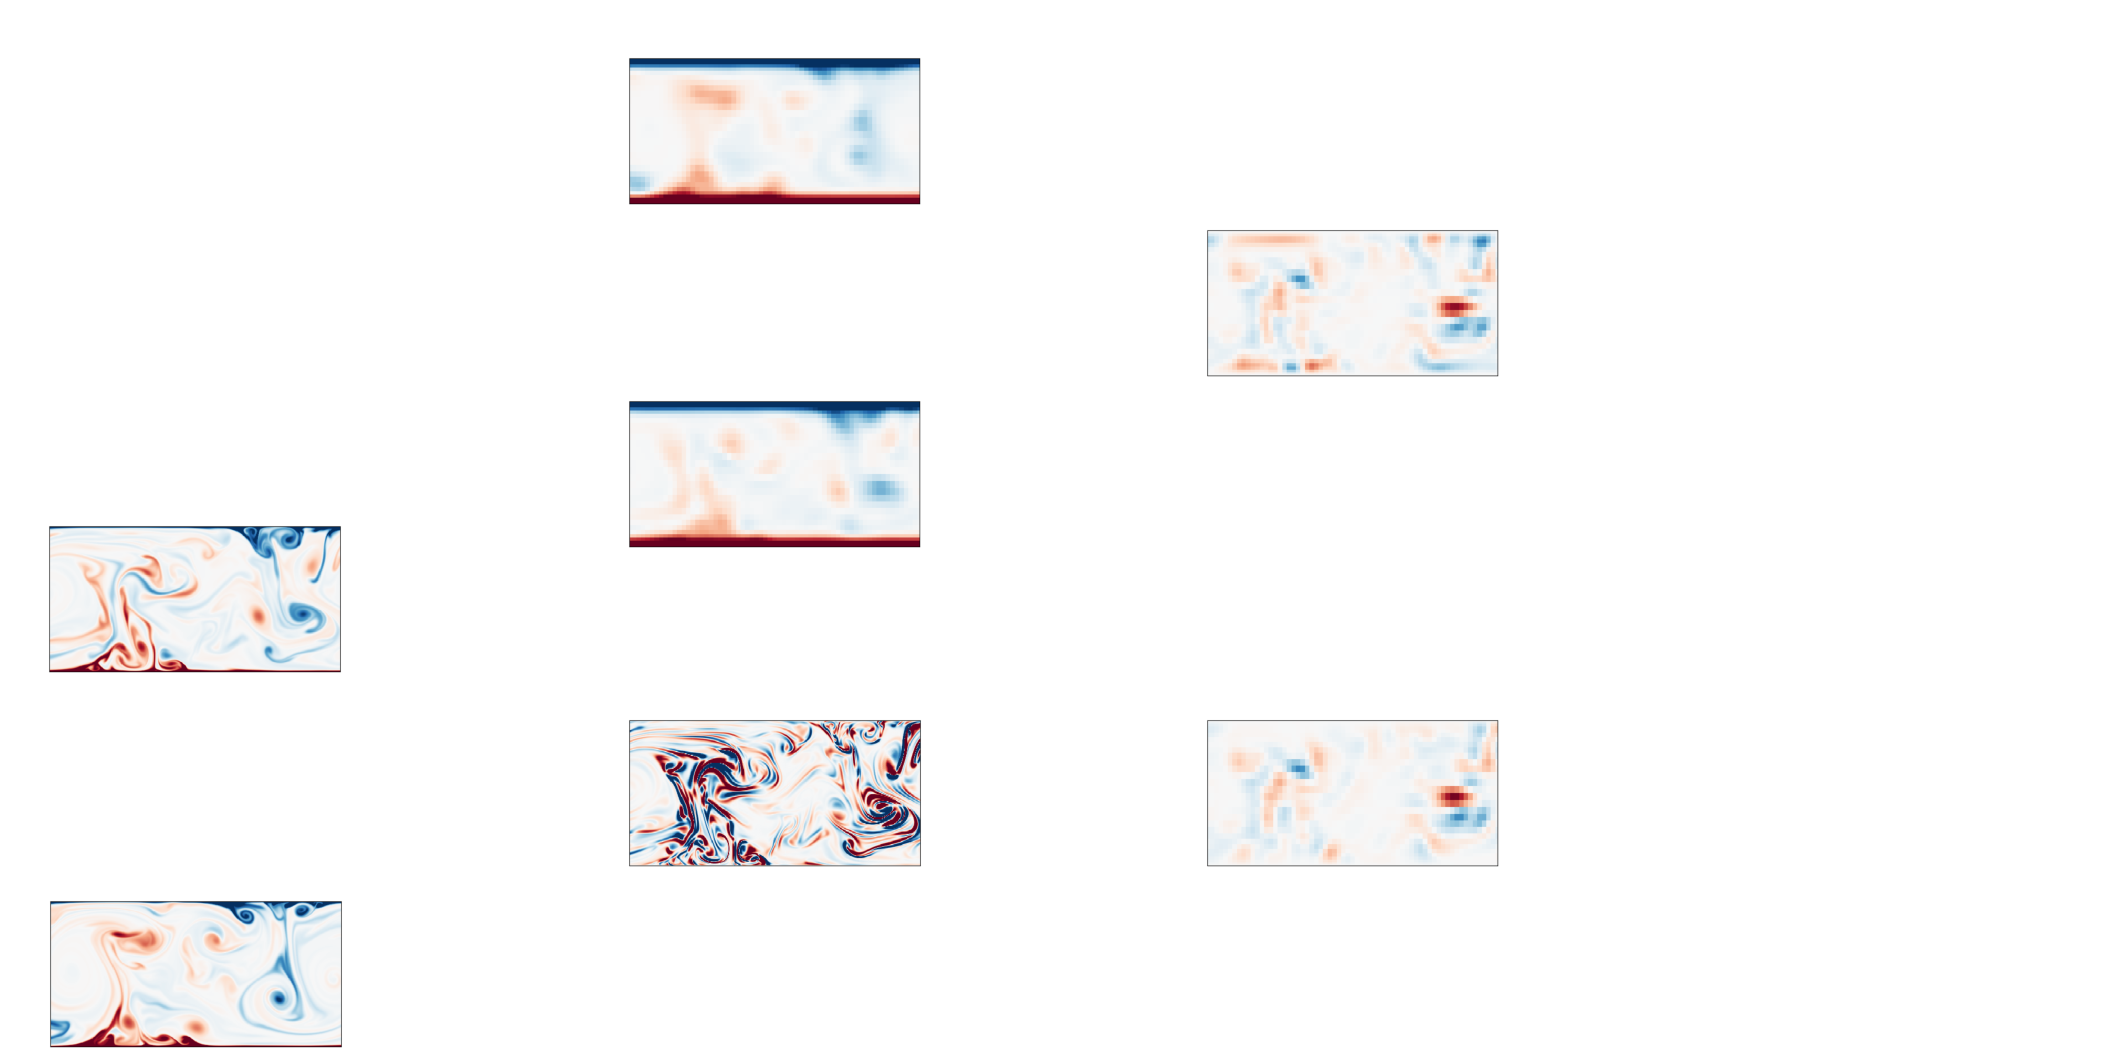
\includegraphics[width=\linewidth]{figures/method5.pdf}
\end{frame}

\begin{frame}
\centering
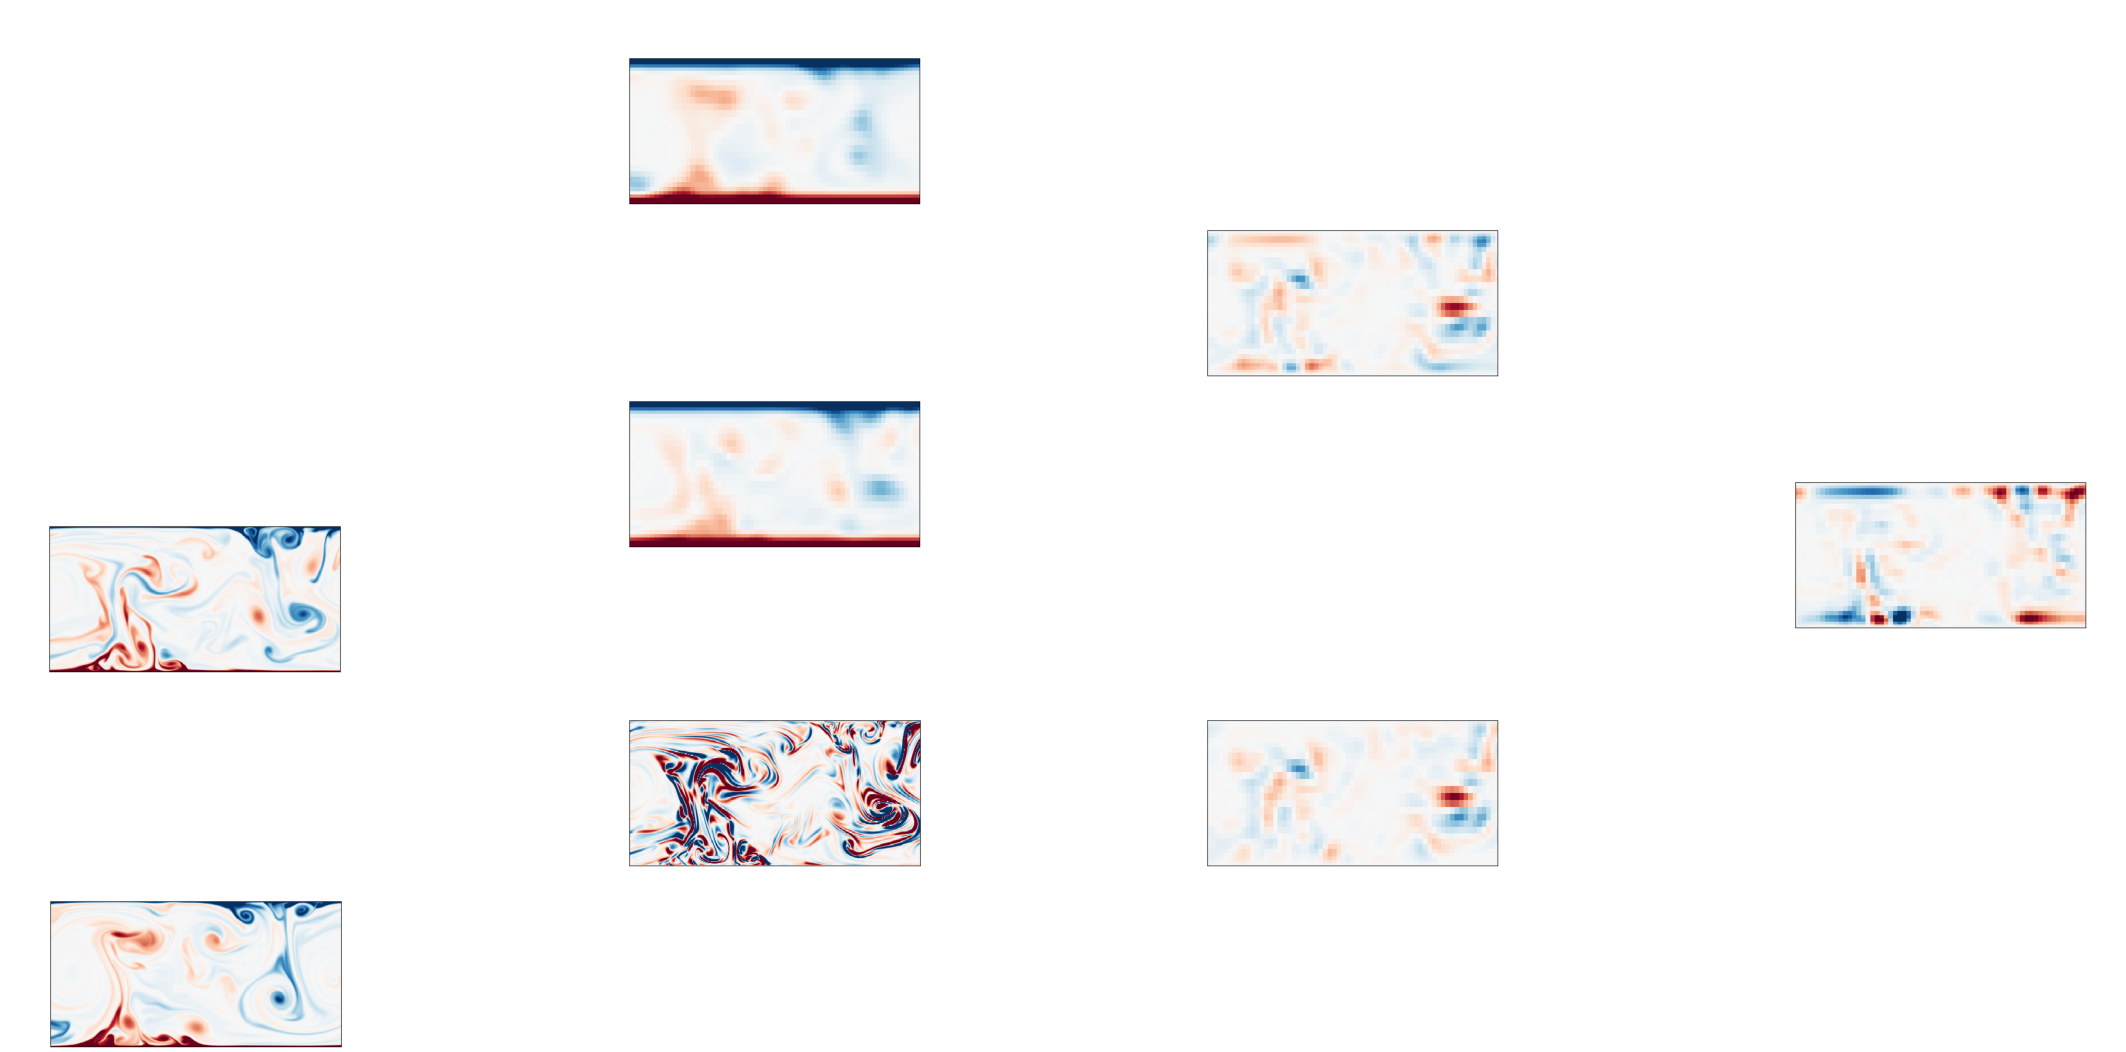
\includegraphics[width=\linewidth]{figures/method6.pdf}
\end{frame}

\section{3. Coarse-graining carefully}

% filtering
\begin{frame}
We need to map the state $\vec{z}$ of the full system to a coarse state
$\vec{x} = \langle \vec{z} \rangle$ that the coarse model sees.

\vspace{20pt}
The definition of $\langle \cdot \rangle$ is up to us (!) and our choice
can strongly affect the results.
\end{frame}

\begin{frame}
The coarse-grained fields must:
\vspace{5pt}
\begin{itemize}
    \itemsep=10pt
    \item Be well-resolved on the coarse grid
    \item Respect physical constraints:
    \vspace{5pt}
    \begin{itemize}
        \itemsep=5pt
        \item $u(z=0,1) = w(z=0,1) = 0$
        \item $\theta(z=0) = 1/2, \theta(z=1) = -1/2$
        \item $\grad \cdot (u, w) = 0$
    \end{itemize}
\end{itemize}
\end{frame}

\begin{frame}
Obvious (but wrong) choice: average fine fields over each coarse grid-box.
\begin{center}
    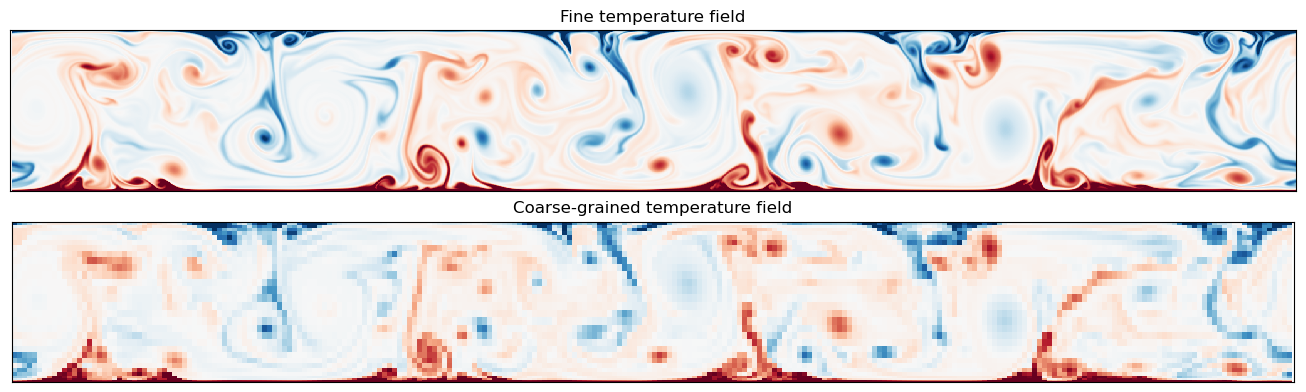
\includegraphics[width=\linewidth]{figures/old_coarse_grain.png}
\end{center}
\begin{itemize}
    \item[$\times$] Not well-resolved on coarse grid
    \item[$\times$] Violates physical constraints
\end{itemize}
\end{frame}

\begin{frame}
Solution: solve the diffusion equations
\begin{align*}
    \pdiff{}{t} \begin{pmatrix} u \\ w \end{pmatrix}
        &= -\grad \pi + \nu \nabla^2 \begin{pmatrix} u \\ w \end{pmatrix} \\[5pt]
    \pdiff{\theta}{t}  &= \kappa \nabla^2 \theta \\[5pt]
    \grad \cdot \begin{pmatrix} u \\ w \end{pmatrix} &= 0
\end{align*}
subject to the required boundary conditions.
\end{frame}

\begin{frame}
\begin{center}
    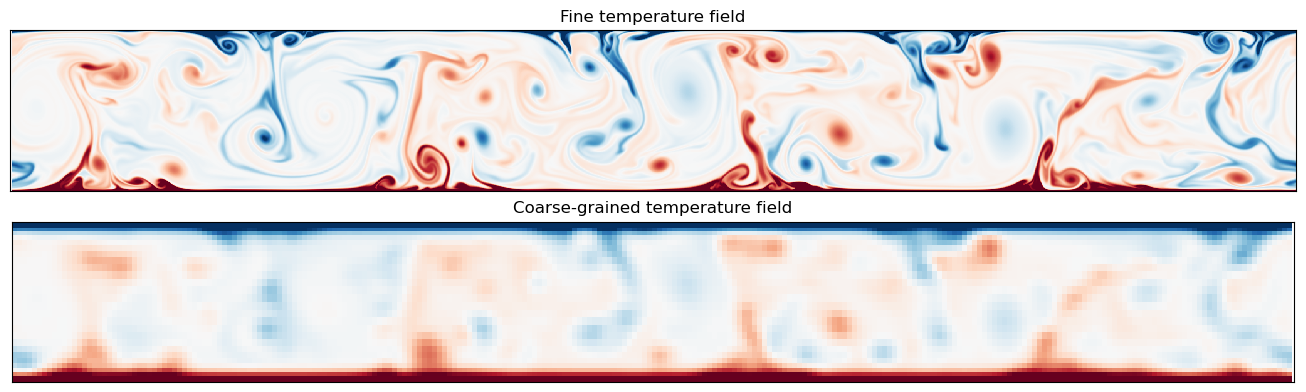
\includegraphics[width=\linewidth]{figures/new_coarse_grain.png}
\end{center}
\begin{itemize}
    \item[$\checkmark$] Well-resolved on coarse grid
    \item[$\checkmark$] Respects physical constraints
\end{itemize}
\end{frame}

\section{4. Can we predict the subgrid tendencies?}

\begin{frame}
\centering
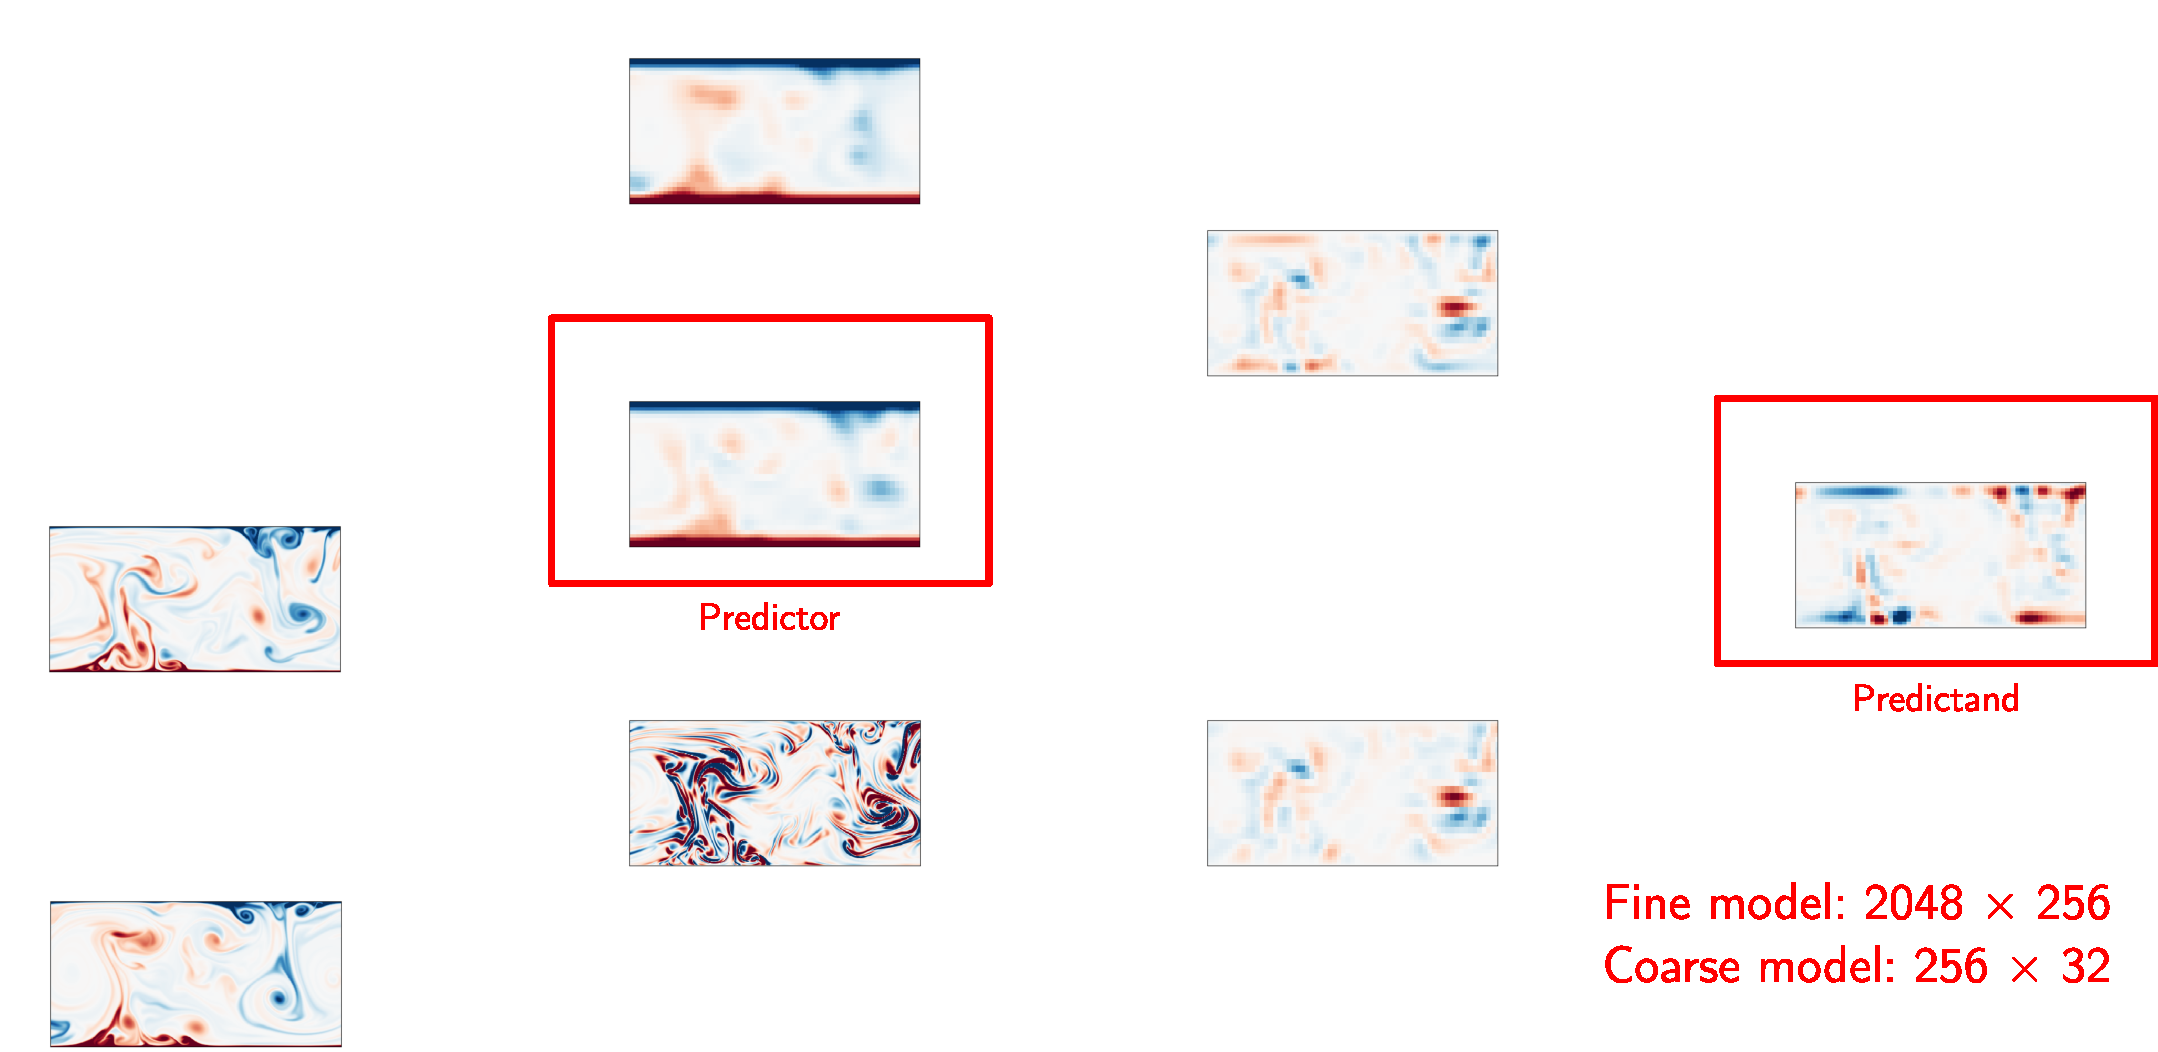
\includegraphics[width=\linewidth]{figures/method7.pdf}
\end{frame}

% histograms
\begin{frame}{Subgrid temperature tendency}
\centering
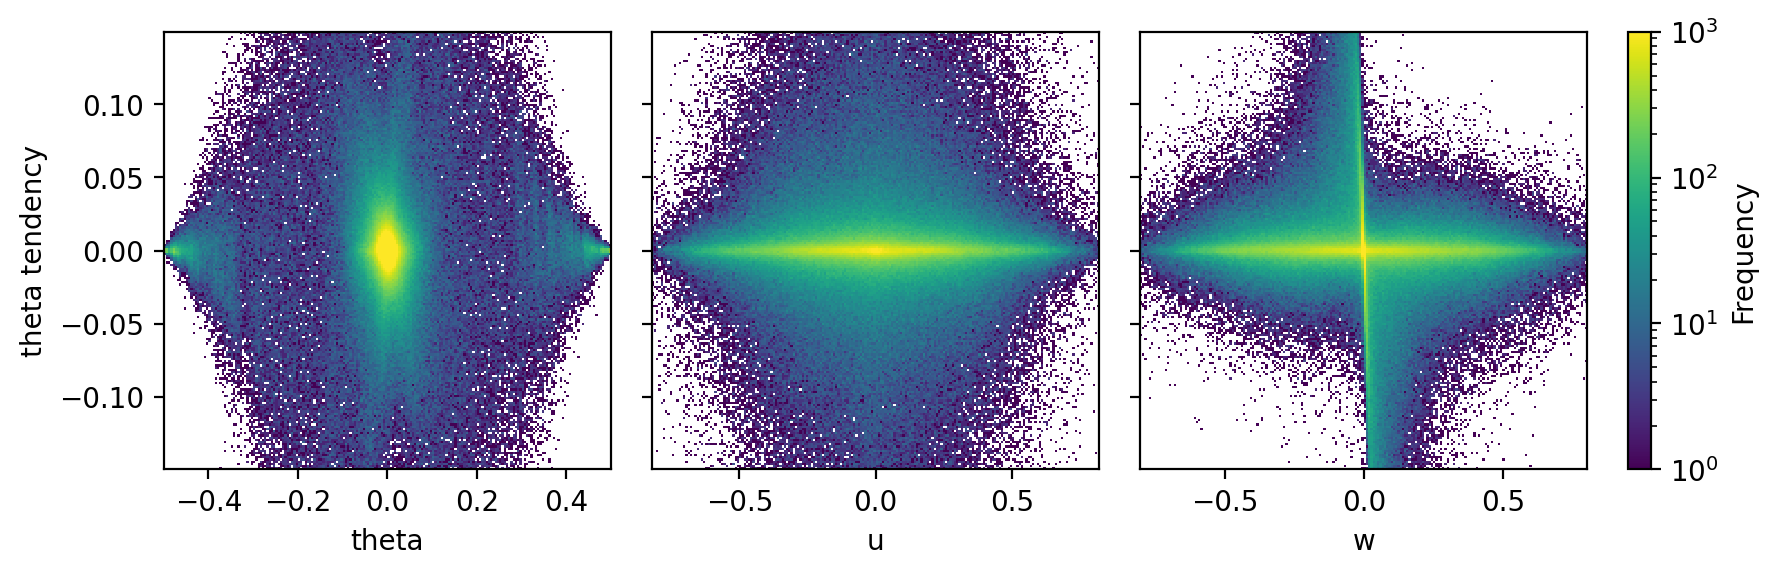
\includegraphics[width=\linewidth]{figures/theta_tend.png}
\end{frame}

\begin{frame}{Subgrid horizontal velocity tendency}
\centering
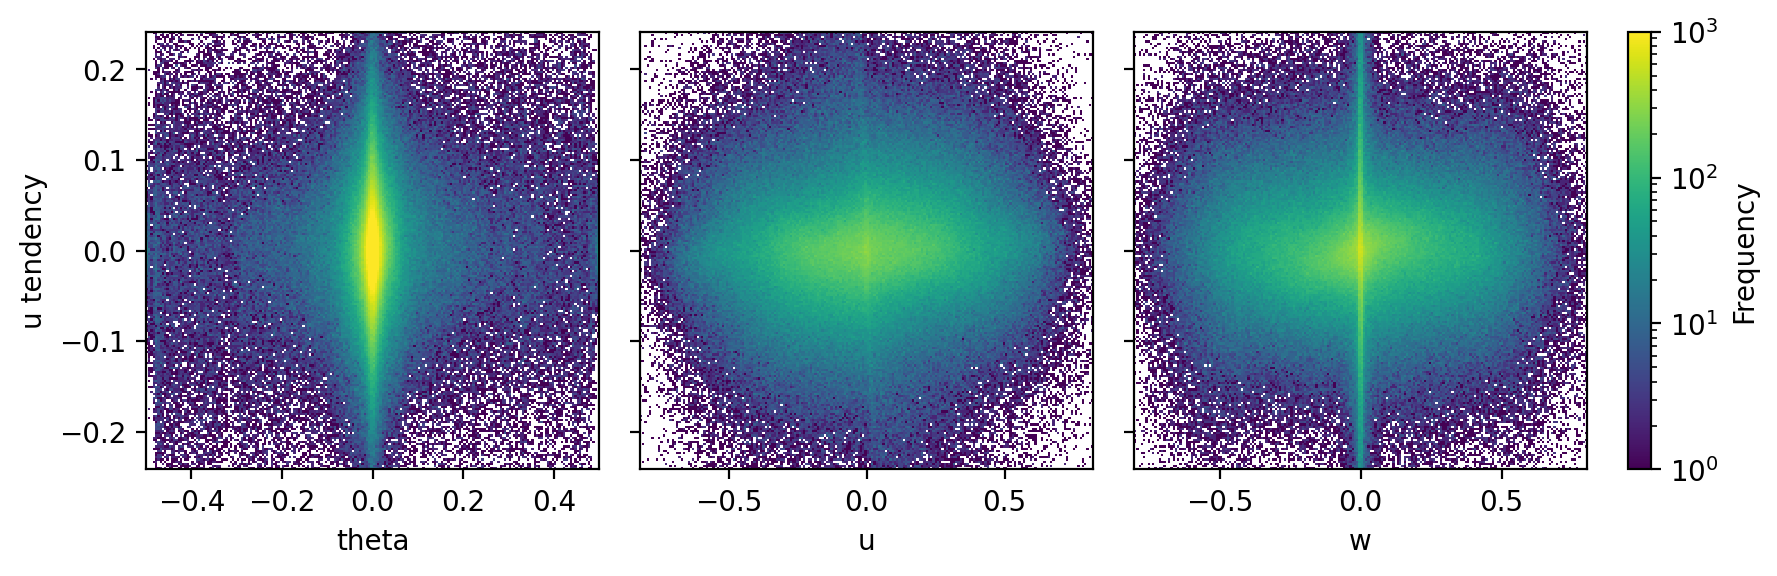
\includegraphics[width=\linewidth]{figures/u_tend.png}
\end{frame}

\begin{frame}{Subgrid vertical velocity tendency}
\centering
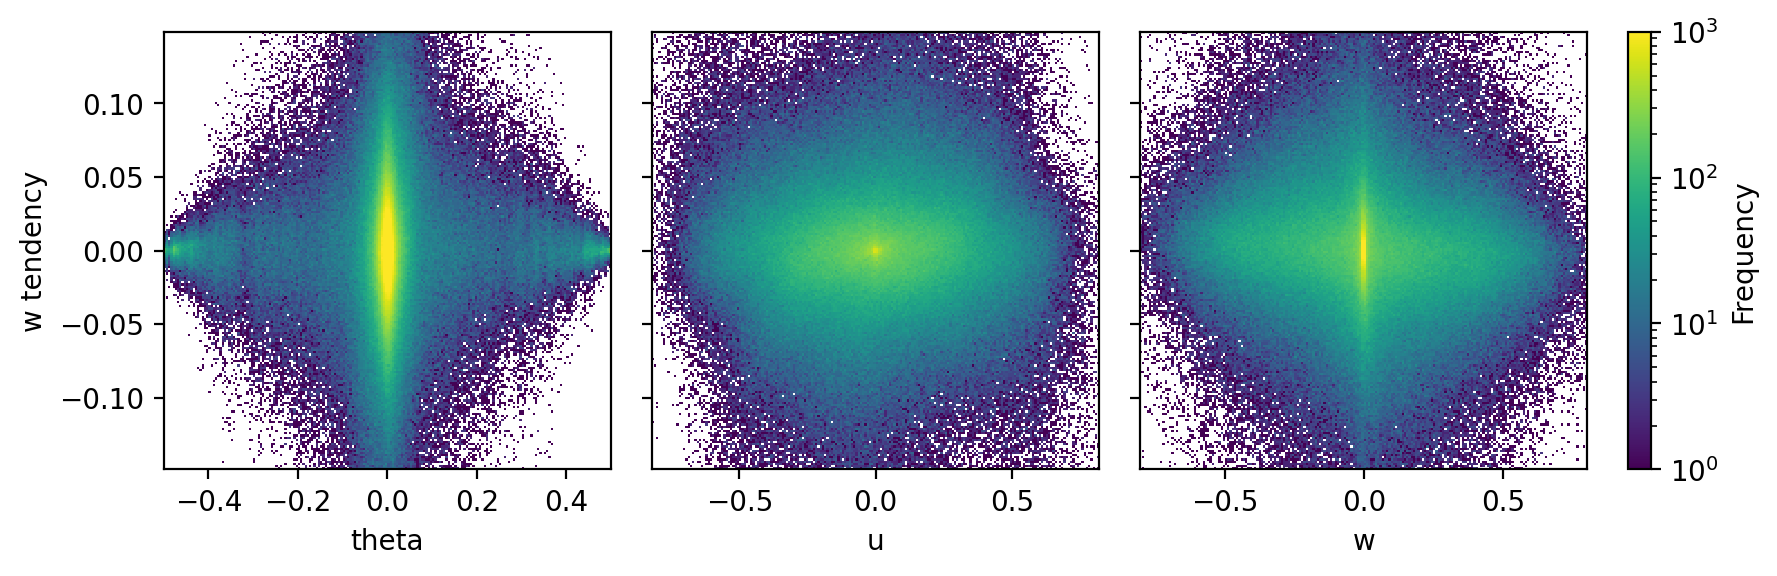
\includegraphics[width=\linewidth]{figures/w_tend.png}
\end{frame}

\begin{frame}{Summary}
\begin{enumerate}
    \itemsep=2em
    \item In principle, one can quantify the effect of small-scale
        processes on the larger scales by coarse-graining high-resolution data.
    \item We implemented this procedure in a 2D model of \rb{} convection.
    \item The choice of coarse-graining method is important.
    \item We found little correlation between subgrid tendencies and the
        coarse variables.
\end{enumerate}
\end{frame}

\section{Next steps?}

\end{document}
